\chapter{Software}
\label{Software}
\section{Überblick}
\section{Steuerung - Magic-Glove}
\label{SW_MagicGlove}
\section{Stromversorgung}
\label{SW_Stromversorgung}
Mit der Software zum Battery Management werden wichtige Punkte geregelt, um ein langes Leben der Akkuzellen zu gewährleisten. Darunter gehören sowohl über- als auch unter- Spannungsschutz sowie ausbalancieren der einzelnen Zellenspannungen beim Laden. \\
Der aktuelle Ladevorgang wird über drei verschiedenen LED’s angezeigt. Dabei zeigen diese den Constant Current (CC), Constant Voltage (CV) und den vollen Zustand (off) an. Diese können als Laden (CC, LED1) Betriebsbereit (CV, LED2) und vollständig geladen (off, LED3) interpretiert werden. 
Das folgende Zustandsdiagramm (Abbildung \ref{fig:statediagrammbatterie}) zeigt den Ablauf der Software auf dem Mikrocontroller.
\begin{figure} [H]
	\centering
	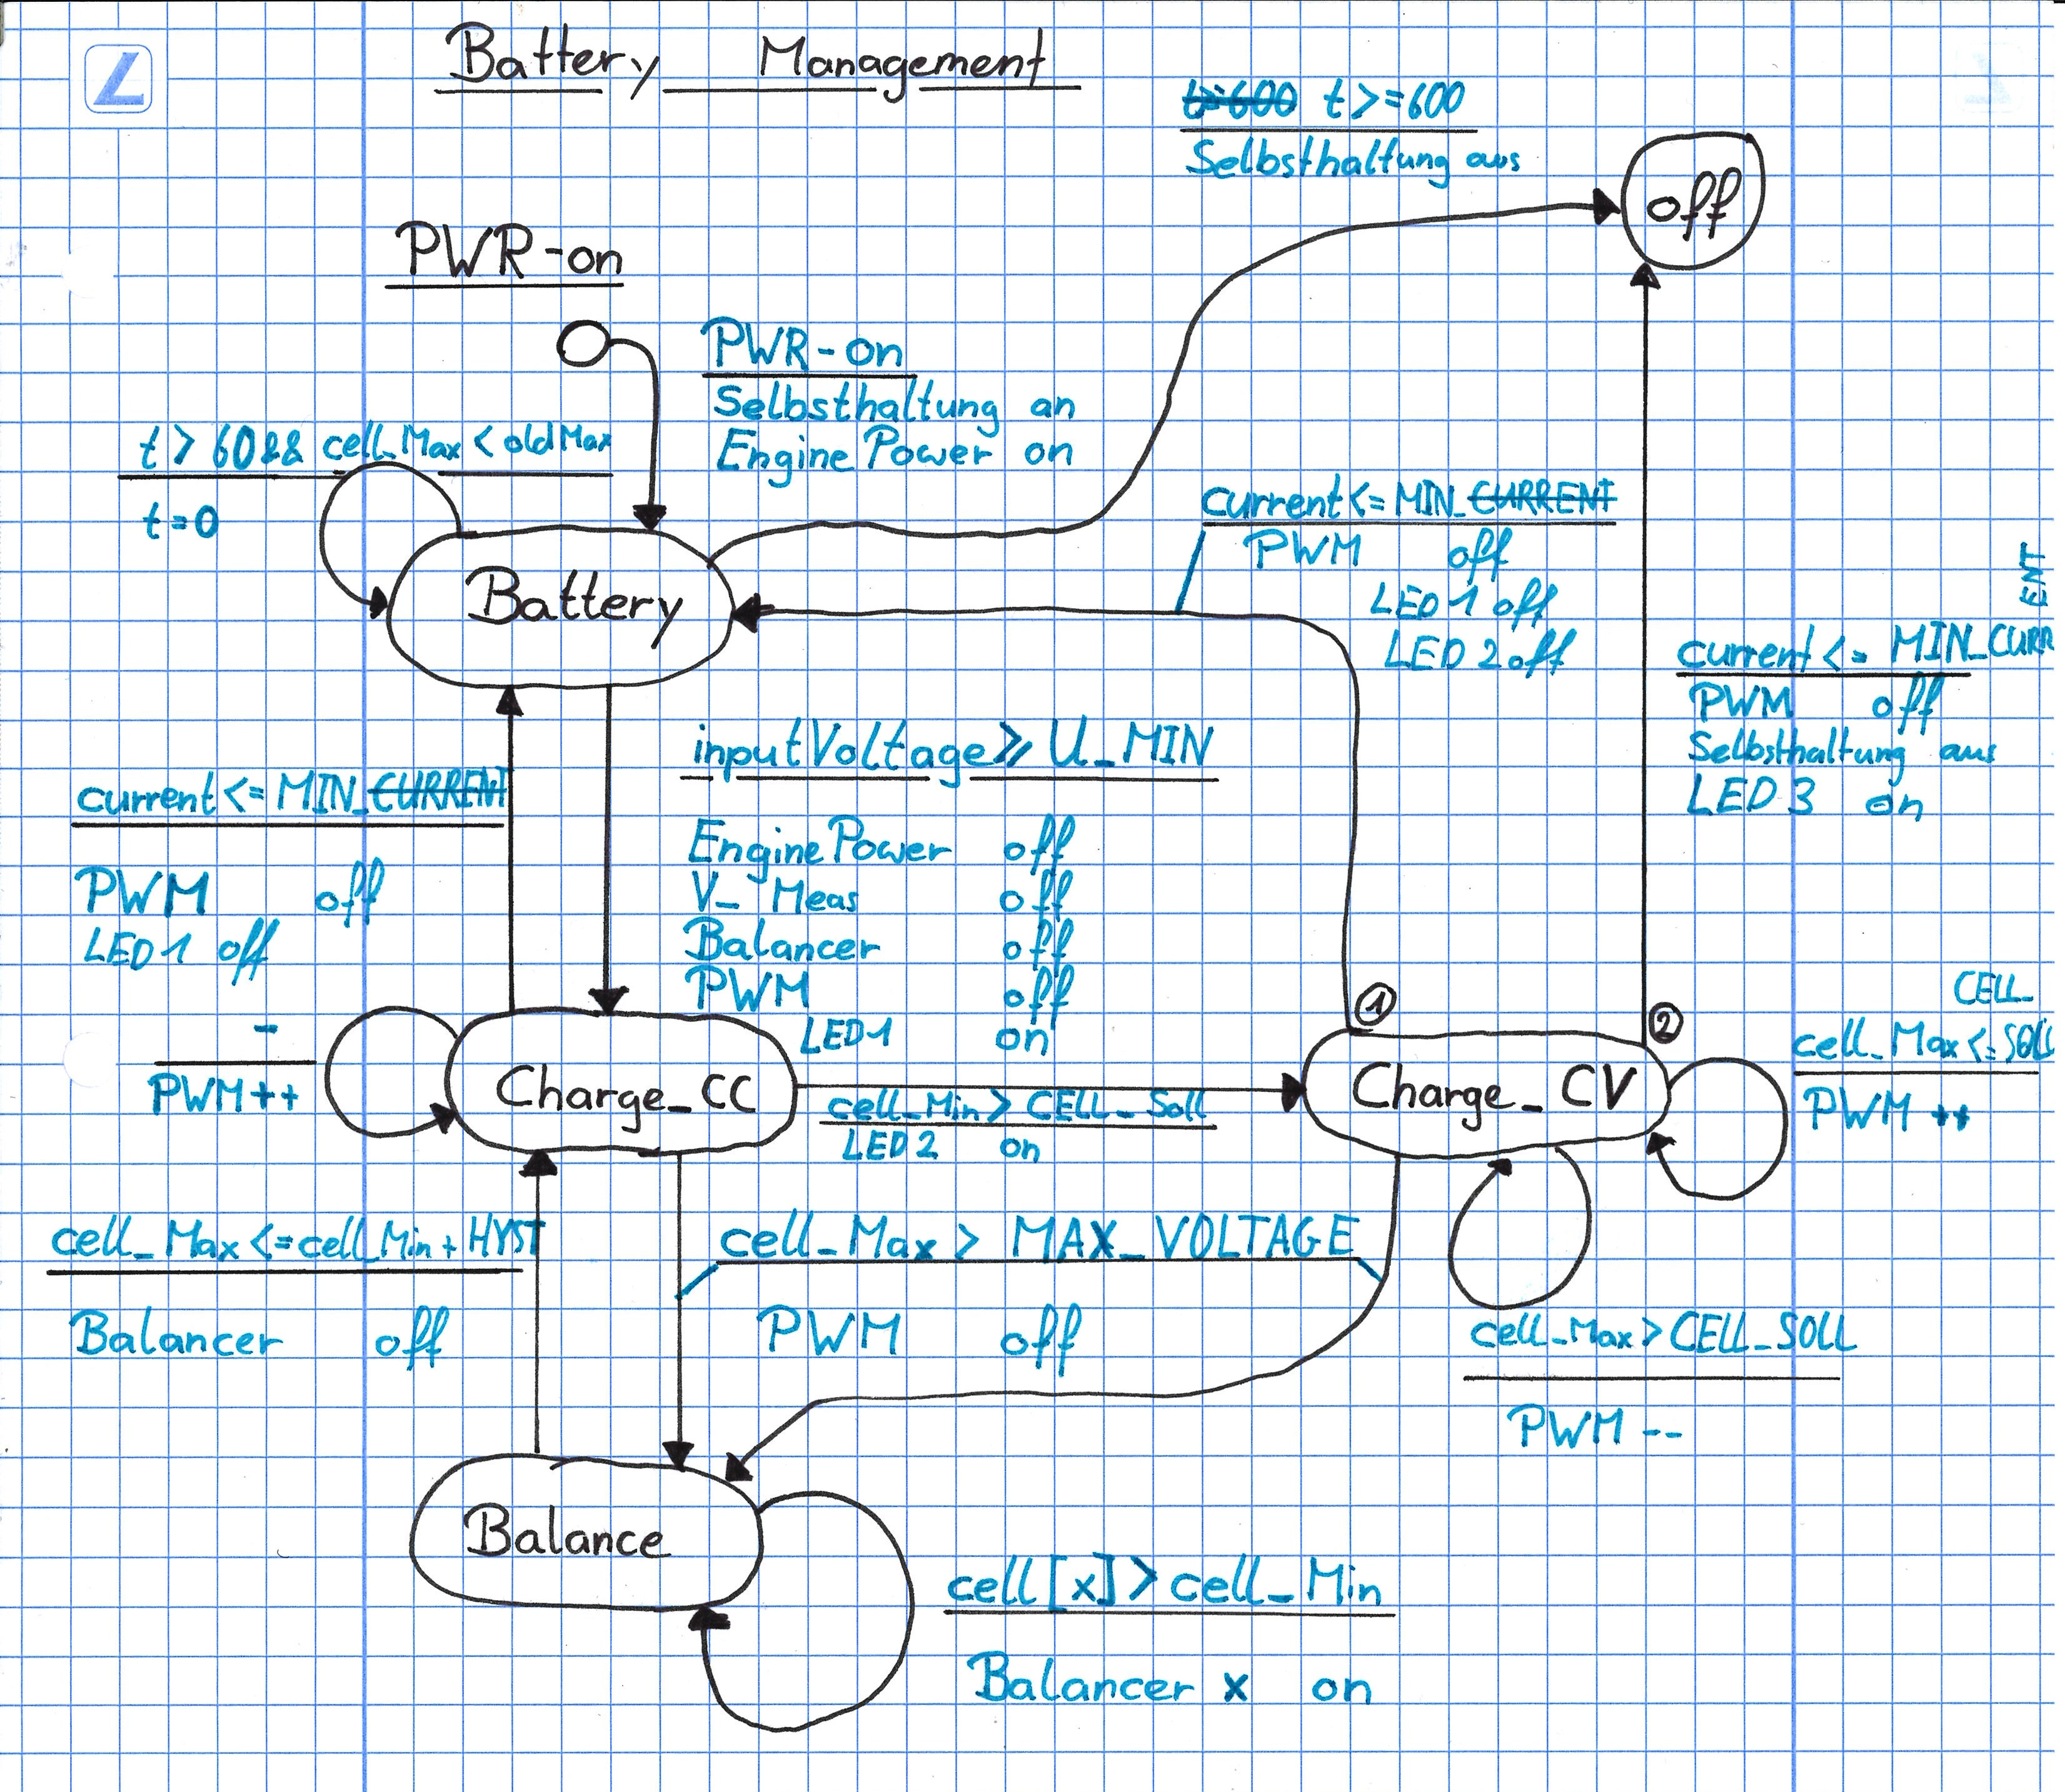
\includegraphics[width=1\linewidth]{images/Statediagramm_Batterie}
	\caption{State Diagramm des Batterie-Management}
	\label{fig:statediagrammbatterie}
\end{figure}
Wie im Hardwareteil schon beschrieben wurde, hält sich der Mikrocontroller mit einer Selbsthaltung in Betrieb. Diese wird jedoch einerseits mit dem Ein- Taster als auch mit der Eingangsspannung des Ladegerätes überbrückt. Wird einer von diesen aktiviert, startet der Mikrocontroller auf und betätigt die Selbsthaltung. \\
Beim Start wird als erstes der \textit{Battery} Zustand geladen. Wenn das Ladekabel nicht angeschlossen ist, wird die Schaltung den Motor mit der benötigten Spannung von den Akkuzellen versorgen. Falls das Board über zehn Minuten nicht gebraucht wird oder sich der Akku der unteren Spannungsgrenze nähert, wird das Board ausgeschaltet. Sobald eine Ladespannung des Ladegeräts angelegt wird, wechselt der Mikrocontroller in den Zustand \textit{Charge\_CC}.\\
In diesem Zustand wird der Strom zunehmend auf die maximalen 5A gebracht und dort konstant gehalten. Dies geschieht durch den Pulsweitenmodulation-Ausgang (PWM-Ausgang) der auf den Schaltregler führt. Je mehr Strom in die Zellen fliesst, desto höher wird deren Spannung. Sobald eine Zelle den Maximalwert von 4.3V überschreitet, wird in den \textit{Balance} Zustand gewechselt. Dort werden alle Zellen auf den Wert der niedrigsten Zelle entladen. Die beiden Zustände werden solange wiederholt, bis sich die  Spannung der niedrigsten Zelle über der Soll Spannung befindet.  Danach wird in den nächsten Zustand \textit{Charge\_CV} gewechselt. \\
Im \textit{Charge\_CV} Zustand wird mit der Regelung des Zuführstromes versucht, die Zellenspannung weiterhin auf dem Sollwert von 4.15V zu halten. Dieser Strom nimmt mit der immer weiter fortschreitenden Aufladung der Zellen kontinuierlich ab, bis schliesslich ein unterer Grenzwert von XXmA \todo{xxx mA} erreicht wird. An diesem Punkt gilt der Akku als voll geladen und wechselt in den Zustand \textit{Off}.
Anders als vielleicht zuerst angenommen bleibt das Board dank der Überbrückung der Selbsthaltung aktiv und zeigt durch die 3 leuchtenden LED’s an, dass der Akku voll aufgeladen ist. Sobald  die Spannung des Ladegeräts abfällt, fällt auch die Selbsthaltung ab. Somit ist das Board komplett ausgeschaltet.
\\\\
Ein weiterer Schwerpunkt der Software war die Berechnung der Spannungen der einzelnen Zellen. Die Zellen sind seriell miteinander verbunden. Somit addieren sich die Spannungen an den Ausgängen jeder Zelle bis auf 24,9V auf der sechsten Zelle. Da der AD-Wandler des Mikrocontroller nur zwischen 0 und 5 Volt messen kann, müssen die Ausgänge der Zellen mit einem Spannungsteiler mit dem Faktor \(\frac 1n\) herunter skaliert werden. Ab der zweiten Spannung sind die Ausgänge jedoch abhängig von den vorherigen Zellen. Um einen richtigen Wert zu erhalten, muss die Differenz inklusive der richtigen Skalierungsfaktoren berechnet werden. Mithilfe dieser Daten kann man für die Spannung der einzelnen Zellen \(cell_0 \dots cell_n\) folgende Formel herleiten:
\begin{equation}
	cell_n = n \cdot ADC(n) - (n-1)\cdot ADC(n-1)
	\label{eq:CellNSpannung}
\end{equation}

\todo{erklärung / Liste der verwendeten Symbole / bedeutung ADC,...}
Die Zellspannungen werden in jedem Durchlauf gemessen und in einem Array abgespeichert. Aus diesen Werten werden die minimale und maximale Spannung berechnet, welche für die verschiedenen Logikabfragen in der Statemachine verwendet werden.

\section{Motoransteuerung}
\label{SW_Motoransteuerung}
\subsection*{Plattform}
Erläuterung der verwendeten SW-Komponenten/Betriebssystem,
\subsection*{Entwicklungsumgebung}
\subsection*{Programmablauf}
Blockschaltmässiger Ablauf der Software
\subsection*{Peripherie}
Verwendete Peripheriegeräte wie Timer, ADC, DMA usw
\subsection*{Modulübersicht}
Jedes Modul wird grob erläutert
\subsection*{Libraries}
Eine Übersicht über alle verwendeten externen Libraries


